% Created 2011-08-05 Fri 13:34
\documentclass{book}


\usepackage{leonine,amsmath,amssymb,amsthm,graphicx,setspace, hyperref}
\renewcommand{\thechapter}{\Roman{chapter}}
\providecommand{\alert}[1]{\textbf{#1}}
\begin{document}



\title{Experimental Results and Notes}
\author{Eric Purdy}
\date{05 August 2011}
\maketitle

\setcounter{tocdepth}{3}
\tableofcontents
\vspace*{1cm}

\chapter{Plan}
\label{sec-1}

\setcounter{section}{-1}
\section{Assembling Datasets}
\label{sec-1_1}
\subsection{Articulator}
\label{sec-1_1_1}
\subsection{Romer}
\label{sec-1_1_2}
\subsection{Weizmann horse dataset}
\label{sec-1_1_3}
\subsection{Hand datasets/ASL alphabet}
\label{sec-1_1_4}
\subsection{LabelMe}
\label{sec-1_1_5}
\subsection{Time series datasets}
\label{sec-1_1_6}
\section{Grammatical Shape Models}
\label{sec-1_2}
\subsection{Compare grammars to markov models}
\label{sec-1_2_1}
\subsection{Compare grammars to procrustes / watson / bingham as baseline}
\label{sec-1_2_2}
\subsection{Build interesting grammars by hand}
\label{sec-1_2_3}
\subsection{Build interesting and valid grammars from shapetrees}
\label{sec-1_2_4}
\subsection{Figure out how to deal with variation in length}
\label{sec-1_2_5}
\subsection{Have good shape models using more complex grammars}
\label{sec-1_2_6}
\section{Parsing}
\label{sec-1_3}
\subsection{Recover a 1-1 correspondence with misleading intermediate points}
\label{sec-1_3_1}
\subsection{Recover a correspondence with extra intermediate points}
\label{sec-1_3_2}
\subsection{Recover a correspondence where some points are missing}
\label{sec-1_3_3}
\subsection{Recover a correspondence with both extra points and missing points}
\label{sec-1_3_4}
\subsection{Given hand-built rich grammar, choose correct structure}
\label{sec-1_3_5}
\section{EM}
\label{sec-1_4}
\subsection{Simple tuning of hand-built grammar with curves of constant length}
\label{sec-1_4_1}
\subsection{Tuning with multiple midpoints, and curves of constant length}
\label{sec-1_4_2}
\subsection{Tuning with curves of variable length}
\label{sec-1_4_3}
\subsection{Tune rich grammars correctly with EM}
\label{sec-1_4_4}
\subsection{Show that EM fails given bad parses}
\label{sec-1_4_5}
\section{Parsing in Cluttered Images}
\label{sec-1_5}
\subsection{Embed a known curve in the 2D parsing problem}
\label{sec-1_5_1}
\subsection{Generate a very clean image and parse}
\label{sec-1_5_2}
\subsection{Find a shape in an actual image}
\label{sec-1_5_3}
\section{Using SDF's in Other Domains}
\label{sec-1_6}
\subsection{Improve on time-series classification with SDF's}
\label{sec-1_6_1}
\section{Learning Structure}
\label{sec-1_7}
\subsection{Figure out optimal single-example grammar}
\label{sec-1_7_1}
\subsection{Implement Merge and Replace}
\label{sec-1_7_2}
\subsection{Implement Merge and Replace KL heuristics}
\label{sec-1_7_3}
\subsection{Use Merge and Replace to search for good grammar}
\label{sec-1_7_4}
\subsection{Figure out how to optimally incorporate new samples}
\label{sec-1_7_5}
\section{Learning Texture}
\label{sec-1_8}
\subsection{Learn a texture-only grammar}
\label{sec-1_8_1}
\subsection{Learn a grammar that combines global shape with local texture}
\label{sec-1_8_2}
\chapter{Results}
\label{sec-2}

\setcounter{section}{-1}
\section{Assembling Datasets}
\label{sec-2_1}
\subsection{Romer}
\label{sec-2_1_1}

\begin{itemize}
\item We have hand-annotated a simplified version of Romer by
    hand-marking 27 points on a number of images
\end{itemize}
%\% \#+CAPTION:    Hand-annotated simplified Romer dataset
%\% \#+ATTR_\LaTeX{}: width=6in placement=[h!]
\includegraphics[width=4in]{./0.datasets/romer/output.d/romerI.eps}

\begin{itemize}
\item Also have the ``ground-truth'' curves that come from diffing images
    with the background, although they are actually quite messy
\end{itemize}
%\% \#+CAPTION:    ``Ground truth'' curves from Romer dataset
\includegraphics[width=4in]{./0.datasets/romer/output.d/romerII.eps}
\begin{itemize}
\item The images themselves
\end{itemize}
\section{Grammatical Shape Models}
\label{sec-2_2}
\subsection{Make sure Watson distribution is reasonable}
\label{sec-2_2_1}


In the following experiments, we select a random triangle (by using a
Gaussian in Bookstein coordinates). We then draw 20 samples from the
Watson distribution centered at this triangle (using 30 for the
concentration parameter of the Watson). We then reestimate the Watson
distribution from the samples.

This is a less noisy version of the learning task that EM faces when
refitting the midpoint distributions of a grammar from 20 samples.
\begin{itemize}

\item Round 1\\
\label{sec-2_2_1_1}%
\includegraphics[width=4in]{./1.grammars/test_watson/output.d/watson.1.true.eps}

\includegraphics[width=4in]{./1.grammars/test_watson/output.d/watson.1.samples.eps}

On the left, the original triangle, on the right, the estimated triangle.

\includegraphics[width=4in]{./1.grammars/test_watson/output.d/watson.1.est.eps}


\item Round 2\\
\label{sec-2_2_1_2}%
\includegraphics[width=4in]{./1.grammars/test_watson/output.d/watson.2.true.eps}

\includegraphics[width=4in]{./1.grammars/test_watson/output.d/watson.2.samples.eps}

On the left, the original triangle, on the right, the estimated triangle.

\includegraphics[width=4in]{./1.grammars/test_watson/output.d/watson.2.est.eps}


\item Round 3\\
\label{sec-2_2_1_3}%
\includegraphics[width=4in]{./1.grammars/test_watson/output.d/watson.3.true.eps}

\includegraphics[width=4in]{./1.grammars/test_watson/output.d/watson.3.samples.eps}

On the left, the original triangle, on the right, the estimated triangle.

\includegraphics[width=4in]{./1.grammars/test_watson/output.d/watson.3.est.eps}


\item Round 4\\
\label{sec-2_2_1_4}%
\includegraphics[width=4in]{./1.grammars/test_watson/output.d/watson.4.true.eps}

\includegraphics[width=4in]{./1.grammars/test_watson/output.d/watson.4.samples.eps}

On the left, the original triangle, on the right, the estimated triangle.

\includegraphics[width=4in]{./1.grammars/test_watson/output.d/watson.4.est.eps}


\item Round 5\\
\label{sec-2_2_1_5}%
\includegraphics[width=4in]{./1.grammars/test_watson/output.d/watson.5.true.eps}

\includegraphics[width=4in]{./1.grammars/test_watson/output.d/watson.5.samples.eps}

On the left, the original triangle, on the right, the estimated triangle.

\includegraphics[width=4in]{./1.grammars/test_watson/output.d/watson.5.est.eps}

\end{itemize} % ends low level
\subsection{Build an interesting grammar by hand}
\label{sec-2_2_2}


Here we are drawing a grammar. We have built this grammar by hand, by
taking the following curve, and specifying a decomposition of it:

%\% \#+CAPTION:    The initial curve
\includegraphics[height=2in]{./1.grammars/hand_built/output.d/hand_built_curve.eps}

Here is the grammar:

Here are some samples from the grammar:

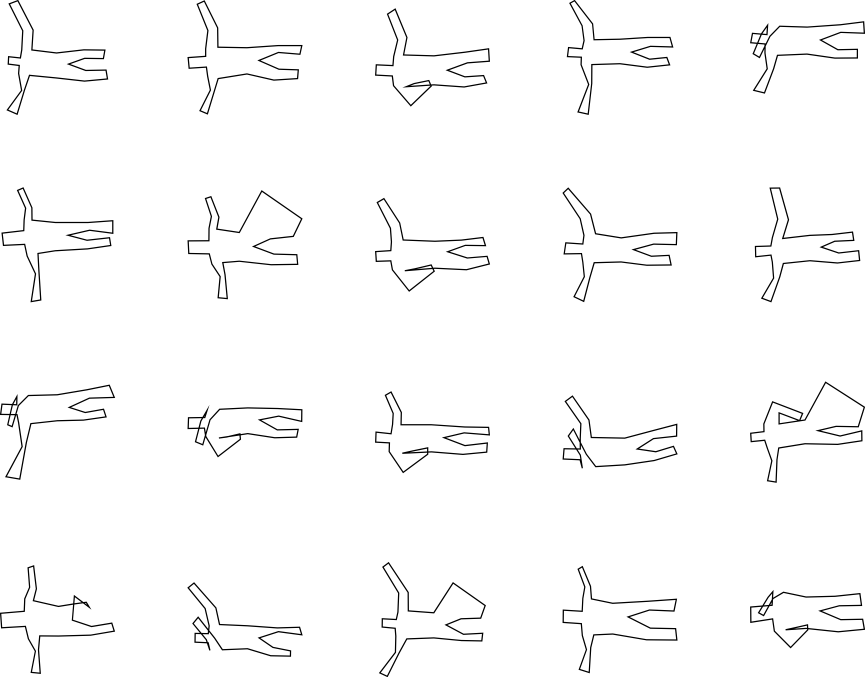
\includegraphics[width=6in]{output/3.learning/incremental/gram.19.d/samples.png}


\section{Parsing}
\label{sec-2_3}
\subsection{One-to-one}
\label{sec-2_3_1}


Here we have two curves given by hand-annotation of the Romer
dataset. We build a grammar from the curve on the left, using a
hand-built set of constituents. We then parse the curve on the right,
and show the Viterbi parse by showing the correspondences between the
two curves.

Because there are no missing or extra points, this is straightforward.

%\% \#+CAPTION:    On the left, the model curve. On the right, the parsed curve
\includegraphics[width=6in]{./2.parsing/one_to_one/output.d/parse.eps}
\subsection{Recover a correspondence with extra intermediate points}
\label{sec-2_3_2}


We build a grammar from a single example from the hand-annotated Romer
dataset, and use it to parse a curve from the ground-truth Romer
dataset. We successfully recover a very reasonable correspondence.

\begin{figure}[htb]
\centering
\includegraphics[width=6in]{./2.parsing/longer_curves/output.d/parse.eps}
\caption{On the left, the model curve. On the right, the parsed curve}
\end{figure}


\begin{itemize}
\item The ground-truth Romer curve has more intermediate points, so this
    demonstrates that our grammar construction and parsing algorithm
    deal well with additional intermediate points. The grammar must
    have lengthening rules, but doesn't need shortening rules.
\end{itemize}
\subsection{Recover a correspondence where some points are missing}
\label{sec-2_3_3}

  Here we build a grammar from a ground-truth Romer curve, and try to
  parse one of the (much shorter) hand-annotated Romer curves. We can
  safely assume that every point in the parsed curve has a
  corresponding one in the example curve, which is the reverse of the
  previous experiments.

  In order to do this successfully, the grammar needs shortening
  rules, but not lengthening rules.

%\% \#+CAPTION:    On the left, the model curve. On the right, the parsed curve
\includegraphics[width=6in]{./2.parsing/shorter_curves/output.d/parse_00.eps}

\begin{itemize}
\item This is really quite bad. We are using a pretty bad SDF to
    initialize the grammar, so maybe that is why.
\item It is somewhat troubling that it does this badly, though. Let us
    try it again with less geometric variation.
\end{itemize}

%\% \#+CAPTION:    On the left, the model curve. On the right, the parsed curve
\includegraphics[width=6in]{./2.parsing/shorter_curves/output.d/parse_80.eps}


\begin{itemize}
\item This is basically correct, although the fine details are not very
    good looking. This is probably because of the SDF. The shortening
    rules only allow the parser to chop off constituents. If the
    constituents look bad, then the parse will look bad.
\end{itemize}
\section{EM}
\label{sec-2_4}
\subsection{Simple tuning of hand-built grammar with curves of constant length}
\label{sec-2_4_1}

Here is our example curve, from which we build a grammar with hand-chosen rules.

%\% \#+CAPTION:    Here is our example curve, from which we build a grammar with hand-chosen rules.

\includegraphics[width=4in]{./3.em/simple_tuning/output.d/examples.eps}

Here are our training curves:

%\% \#+CAPTION:    Here are our training curves:
\includegraphics[width=4in]{./3.em/simple_tuning/output.d/training.eps}
\begin{itemize}

\item Initial\\
\label{sec-2_4_1_1}%
Here are some samples from the grammar:

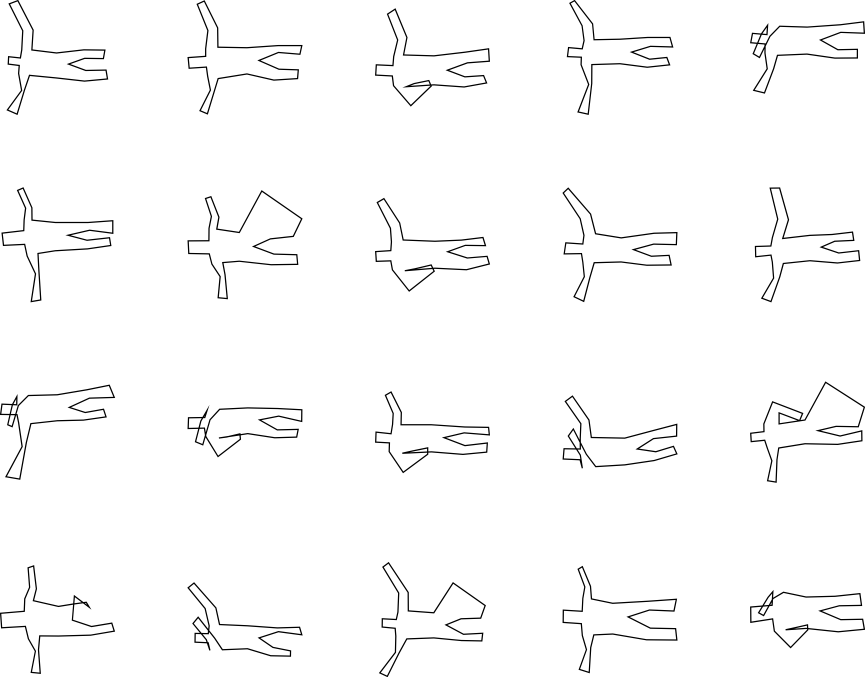
\includegraphics[width=6in]{output/3.learning/incremental/gram.19.d/samples.png}



\item Round 1\\
\label{sec-2_4_1_2}%
Here are some samples from the grammar:

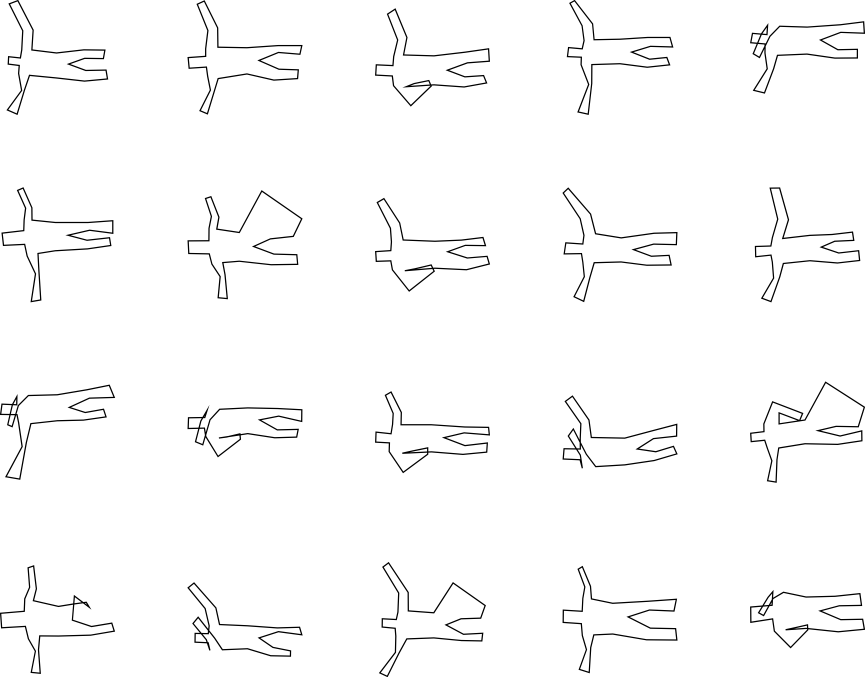
\includegraphics[width=6in]{output/3.learning/incremental/gram.19.d/samples.png}



\item Round 2\\
\label{sec-2_4_1_3}%
Here are some samples from the grammar:

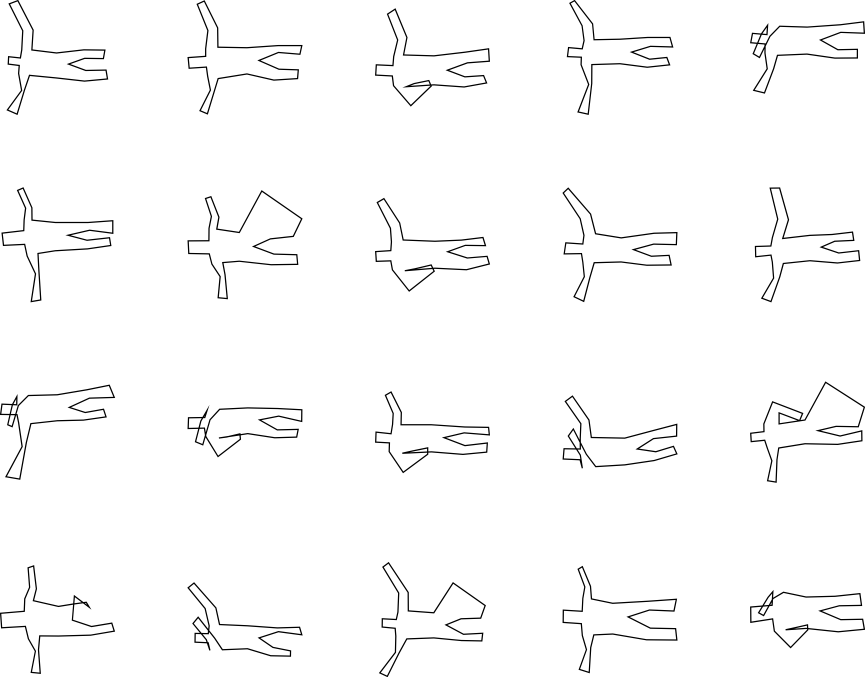
\includegraphics[width=6in]{output/3.learning/incremental/gram.19.d/samples.png}



\end{itemize} % ends low level
\subsection{Tuning with multiple midpoints, and curves of constant length}
\label{sec-2_4_2}


Here is our example curve, from which we build a grammar with
hand-chosen rules. We then enrich the grammar by adding in several
copies of each rule, with jittered midpoints.

%\% \#+CAPTION: Here is our example curve, from which we build a grammar
%\% \#with hand-chosen rules. We then enrich the grammar by adding in
%\% \#several copies of each rule, with jittered midpoints

\includegraphics[width=3in]{./3.em/multi_tuning/output.d/examples.eps}

Here are our training curves:

%\% \#+CAPTION:    Here are our training curves:
\includegraphics[width=3in]{./3.em/multi_tuning/output.d/training.eps}
\begin{itemize}

\item Initial\\
\label{sec-2_4_2_1}%
Here are some samples from the grammar:

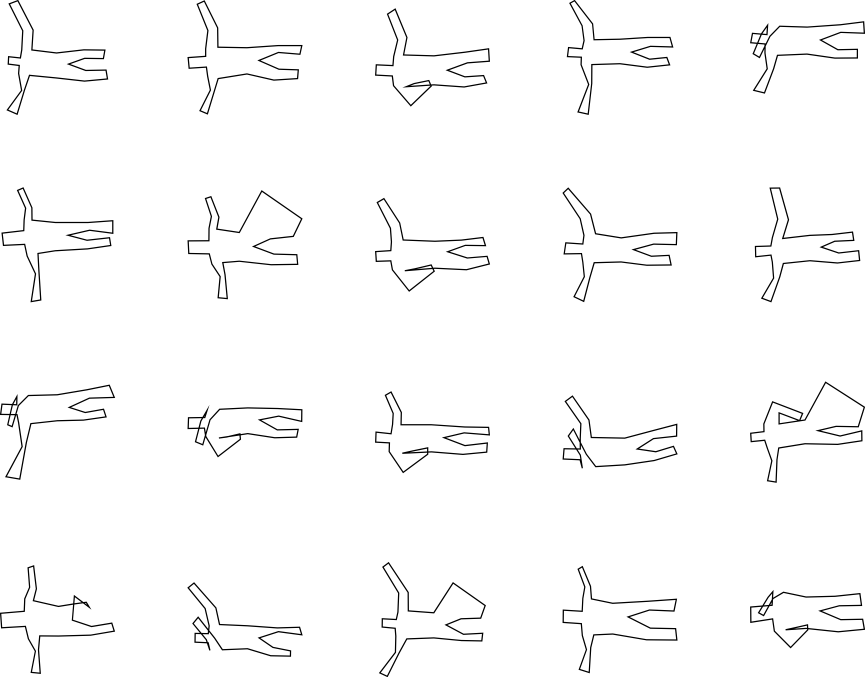
\includegraphics[width=6in]{output/3.learning/incremental/gram.19.d/samples.png}



\item Round 1\\
\label{sec-2_4_2_2}%
Here are some samples from the grammar:

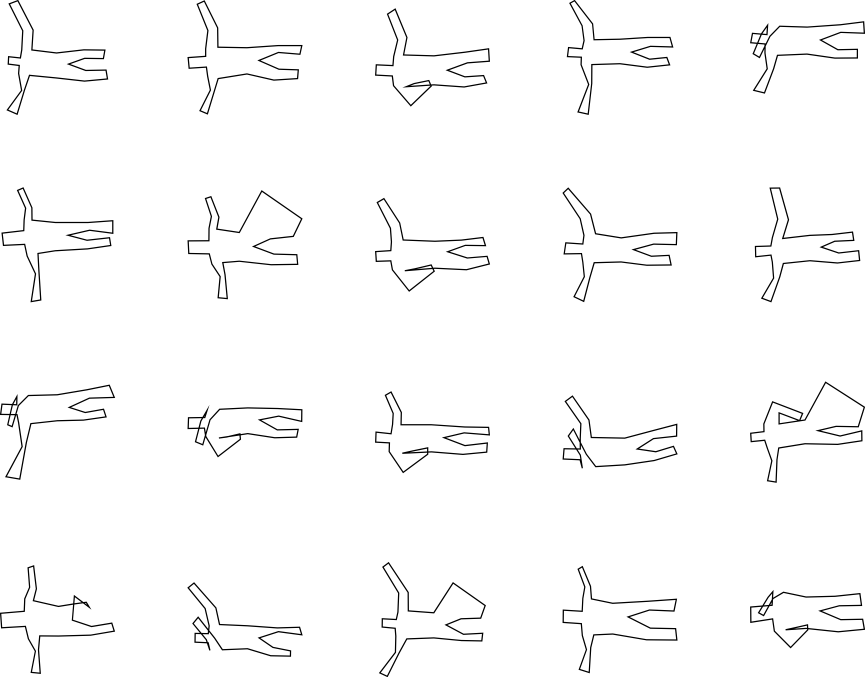
\includegraphics[width=6in]{output/3.learning/incremental/gram.19.d/samples.png}



\item Round 2\\
\label{sec-2_4_2_3}%
Here are some samples from the grammar:

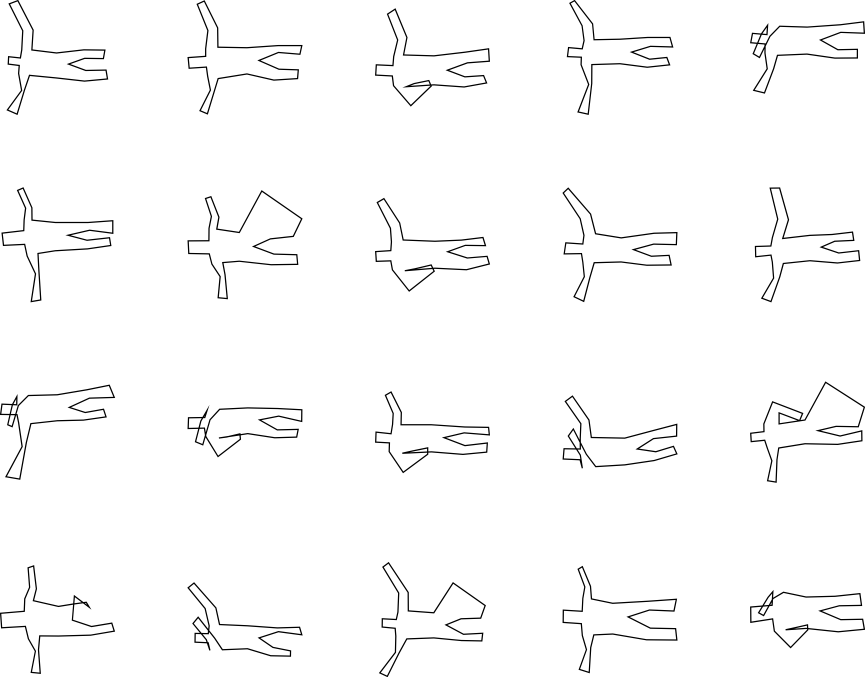
\includegraphics[width=6in]{output/3.learning/incremental/gram.19.d/samples.png}



\item Round 3\\
\label{sec-2_4_2_4}%
Here are some samples from the grammar:

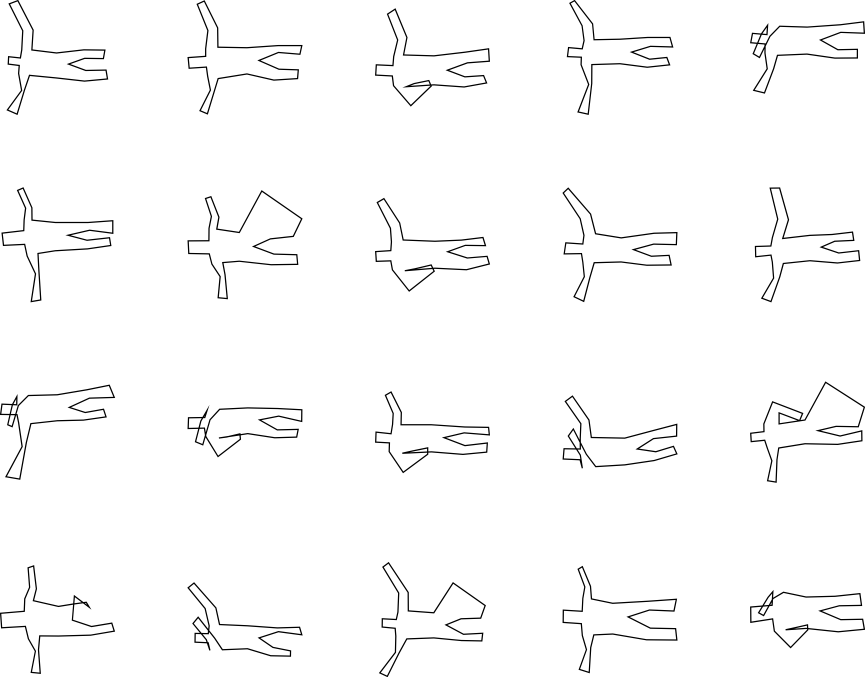
\includegraphics[width=6in]{output/3.learning/incremental/gram.19.d/samples.png}



\item Round 4\\
\label{sec-2_4_2_5}%
Here are some samples from the grammar:

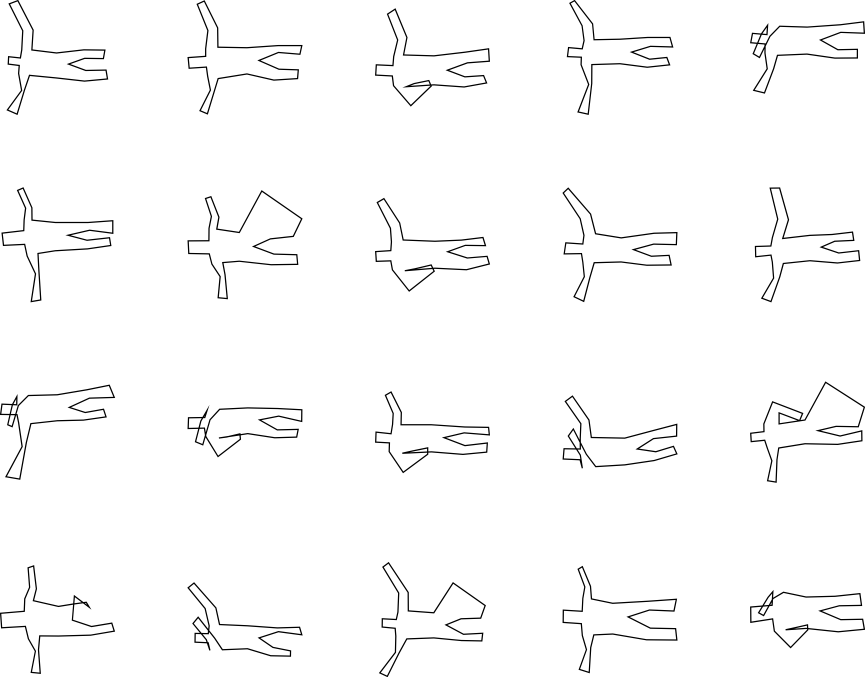
\includegraphics[width=6in]{output/3.learning/incremental/gram.19.d/samples.png}



\item Round 5\\
\label{sec-2_4_2_6}%
Here are some samples from the grammar:

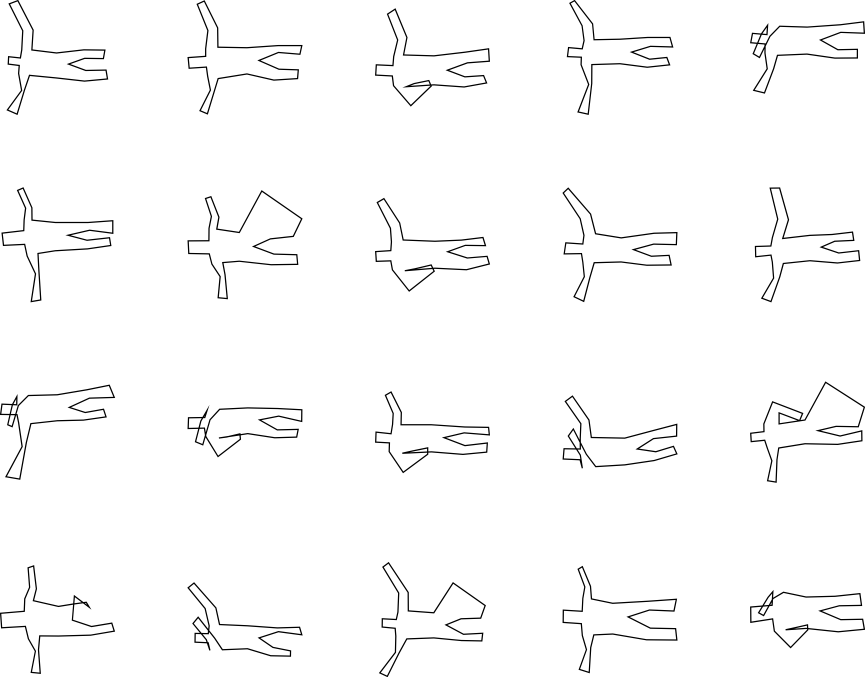
\includegraphics[width=6in]{output/3.learning/incremental/gram.19.d/samples.png}







\end{itemize} % ends low level
\section{Parsing in Cluttered Images}
\label{sec-2_5}
\subsection{Simplified version of the task}
\label{sec-2_5_1}


We build a grammar from a single curve, using a hand-picked
decomposition.


\includegraphics[width=4in]{./4.images/standard_cky/output.d/examples.eps}

We then pick another curve which we wish to parse:

\includegraphics[width=4in]{./4.images/standard_cky/output.d/target.eps}

We build a simple network on a 16x16 grid. We give curve segments a
data cost of 1.0, and short non-curve segments a data cost of 100.0.
Here are the points of the network, with the curve segments shown:

\includegraphics[width=10em]{./4.images/standard_cky/output.d/network.eps}

The parsing algorithm finds the following parse:

\includegraphics[width=10em]{./4.images/standard_cky/output.d/cky.iter6.nt0.eps}
\section{Using SDF's in Other Domains}
\label{sec-2_6}
\section{Learning Structure}
\label{sec-2_7}
\subsection{Figure out optimal single-example grammar}
\label{sec-2_7_1}


We use explicit correspondences to learn the statistically best set of
constituents when building a grammar from a single example.

Note that the arms are found as constituents!

There is a strange issue here, but I've seen it before in other code
and I don't think it's a bug. Converting to Bookstein coordinates
improves the results (or here, the results are more intuitive to me),
even though the Watson distribution shouldn't need this.

Here are the constituents selected by the algorithm:

%\% \#+CAPTION:    Constituents selected.
\includegraphics[width=5in]{./6.structure/constituents/output.d/constituents.eps}
\section{Learning Texture}
\label{sec-2_8}
\subsection{Trying to learn a texture-only grammar}
\label{sec-2_8_1}

\begin{itemize}
\item set up some hierarchy of scales, with decompositions between them

\begin{itemize}
\item would like to use all the data we can get, which means we want
      every length of curve to be close to some scale
\end{itemize}

\item build a grammar from this
\item learn midpoint distributions by going over all pairs of curve
    points and taking the midpoint (and maybe other percentiles) by
    arclength to get triangles
\item sample from it
\item Here are samples from such a grammar, built from every class of
    the Swedish leaf dataset. Some classes are being modeled
    reasonably, some are not.
\end{itemize}

 \includegraphics[width=10em]{./7.texture/scaled_nts/output.d/scaled_nts.1.eps}
\includegraphics[width=10em]{./7.texture/scaled_nts/output.d/scaled_nts_training.1.eps}
\includegraphics[width=10em]{./7.texture/scaled_nts/output.d/scaled_nts.2.eps}
\includegraphics[width=10em]{./7.texture/scaled_nts/output.d/scaled_nts_training.2.eps}
\includegraphics[width=10em]{./7.texture/scaled_nts/output.d/scaled_nts.3.eps}
\includegraphics[width=10em]{./7.texture/scaled_nts/output.d/scaled_nts_training.3.eps}
\includegraphics[width=10em]{./7.texture/scaled_nts/output.d/scaled_nts.4.eps}
\includegraphics[width=10em]{./7.texture/scaled_nts/output.d/scaled_nts_training.4.eps}
\includegraphics[width=10em]{./7.texture/scaled_nts/output.d/scaled_nts.5.eps}
\includegraphics[width=10em]{./7.texture/scaled_nts/output.d/scaled_nts_training.5.eps}
\includegraphics[width=10em]{./7.texture/scaled_nts/output.d/scaled_nts.6.eps}
\includegraphics[width=10em]{./7.texture/scaled_nts/output.d/scaled_nts_training.6.eps}
\includegraphics[width=10em]{./7.texture/scaled_nts/output.d/scaled_nts.7.eps}
\includegraphics[width=10em]{./7.texture/scaled_nts/output.d/scaled_nts_training.7.eps}
\includegraphics[width=10em]{./7.texture/scaled_nts/output.d/scaled_nts.8.eps}
\includegraphics[width=10em]{./7.texture/scaled_nts/output.d/scaled_nts_training.8.eps}
\includegraphics[width=10em]{./7.texture/scaled_nts/output.d/scaled_nts.9.eps}
\includegraphics[width=10em]{./7.texture/scaled_nts/output.d/scaled_nts_training.9.eps}
\includegraphics[width=10em]{./7.texture/scaled_nts/output.d/scaled_nts.10.eps}
\includegraphics[width=10em]{./7.texture/scaled_nts/output.d/scaled_nts_training.10.eps}
\includegraphics[width=10em]{./7.texture/scaled_nts/output.d/scaled_nts.11.eps}
\includegraphics[width=10em]{./7.texture/scaled_nts/output.d/scaled_nts_training.11.eps}
\includegraphics[width=10em]{./7.texture/scaled_nts/output.d/scaled_nts.12.eps}
\includegraphics[width=10em]{./7.texture/scaled_nts/output.d/scaled_nts_training.12.eps}
\includegraphics[width=10em]{./7.texture/scaled_nts/output.d/scaled_nts.13.eps}
\includegraphics[width=10em]{./7.texture/scaled_nts/output.d/scaled_nts_training.13.eps}
\includegraphics[width=10em]{./7.texture/scaled_nts/output.d/scaled_nts.14.eps}
\includegraphics[width=10em]{./7.texture/scaled_nts/output.d/scaled_nts_training.14.eps}
\includegraphics[width=10em]{./7.texture/scaled_nts/output.d/scaled_nts.15.eps}
\includegraphics[width=10em]{./7.texture/scaled_nts/output.d/scaled_nts_training.15.eps}
\chapter{Working notes - front burner (limit 5)}
\label{sec-3}
\section{Multiple jittered midpoints in EM}
\label{sec-3_1}

\begin{itemize}
\item Next step: try upweighting the original midpoint, might keep parses less
    insane (if that helps, it tells us a \textbf{lot} about the weaknesses of
    EM)
\item works sort of OK, need to think about what's going wrong, but
    pretty respectable
\item might also want to use fewer copies, or somehow delete more rules?
\end{itemize}
\section{Adaptive SDF's}
\label{sec-3_2}


\begin{itemize}
\item Next step: unfuck the subsampling code to the point where it will
    give us an intelligent subsampling that has like 8-10 points.
\item do several iterations of subsampling
\item we wrote down a rule in the notebook that keeps the family
    $\theta$-flexible
\item need to figure out what to do with the top-level, it still has 18
    points. Can we actually have that many rules? it would be
    18*17*16? Certainly at least that over 6, which is about 800,
    probably that over 2, about 2400
\item the subsampling algorithm doesn't want to make the curve much coarser
\end{itemize}
\begin{itemize}
\item can decrease the number of rules slightly be only looking at
    relatively balanced ones, that won't exclude many reasonable
    parses
\item for every sub-interval of the top-level, it is either short or
    long. For the long ones, we can add its rules now.
\item For short intervals at the top level, we remember them and use
    them as seeds for the next level
\item At the next level, look at every seed. Sub-intervals of these
    seeds are allowable intervals now. Iterate over all sub-intervals
    of every seed. If they are long enough, add rules now. Otherwise,
    make them seeds for the next level.
\item Try parsing a full Romer curve with the hand-built Romer. Good
    test because it needs to have very good constituents and it needs
    to be very efficient.
\item can we tie the cost function to the original curve throughout, or
    will it be tied to the current approximation? More important for
    length balance terms than data terms, probably
\end{itemize}
\section{2D approximate parsing}
\label{sec-3_3}

\begin{itemize}
\item Next step: Use only straightforward CKY parsing. Start with a very
    coarse grid, say 32x32, so that cubic parsing is not completely
    impossible. Round the target curve to grid points. Embed the curve
    in its Curve.normalize box.
\item Fuzzy cky: we have a hierarchy of curve networks. Each point in a
    given curve network gets mapped to a particular point in the curve
    network above it. We have a maximum distance that is allowed
    between p,q, and r at each level.

    We do parsing as usual at each level (with the constraint that
    p,q,r must be close), and then map the parse table up a level by
    coarsening points.

    questions: how fine should the finest level be? start with 16x16,
    i guess. what is the maximum allowable length? let's say 5 units,
    see what happens
\item Define a hierarchy of increasingly difficult versions of the
    problem
\end{itemize}


\begin{center}
\begin{tabular}{ll}
\hline
 Grammar source           &  Data cost                              \\
\hline
 hand-built               &  take fixed curve, make cost very low   \\
                          &  for segment close to a curve segment,  \\
                          &  very high o/w                          \\
\hline
 automatically generated  &  draw filled curve in black, run canny  \\
                          &  to get edge quality, charge cost       \\
                          &  accordingly                            \\
\hline
                          &  Take image, run canny or PB            \\
\hline
\end{tabular}
\end{center}



\begin{itemize}
\item think about how to only look at midpoints close to the Watson mode
\item can speed up parsing by only considering X$\to$ C$_{\mathrm{p,q}}$ when p and q
    are ``about the right distance apart'' given that we know the global
    scale approximately, and that we know how far apart they tend to
    be relative to that (can answer that by sampling, or learn it)
\item work only with a fixed parse tree for now, since L$\to$ LL was the
    source of more than half our woes. as long as we have $P(X\to
    \ell_{p,q})$ for all $p,q$, and we think that our segments are
    straight, it's fine to do this.
\item think about fuzzy versions of CKY. have notes in the notebook, but
    it's a really terrible problem to think about
\end{itemize}
\section{Structure: Constituency}
\label{sec-3_4}

\begin{itemize}
\item Next step: draw the grammar we selected, show samples
\end{itemize}
\section{Structure: Constituency heuristics}
\label{sec-3_5}


\begin{itemize}
\item Next step: make an experiment for this
\item General thought: if removability is a good constituency test, then
    what tells us that a subcurve is removable? Protuberance obviously
    does, since we can imagine cutting it off at the bottleneck.
\item the triangle decay algorithm is working somewhat interestingly. we
    should think about the super long and skinny triangles; maybe we
    want them as constituents, maybe we don't.
\item How do we turn the triangle decay path into an SDF? If we run the
    decay backwards, it gives a decomposition whose top-most level is
    ambiguous (can break a triangle in three ways), but otherwise
    unambiguous
\item it is a semi-reasonable decomposition, but it acts weirdly around
    certain protuberances. it cannot search over all decompositions of
    a protuberance, only those that correspond to growing it by
    triangles. For some protuberances, the negative triangle check is
    actually preventing the most intuitive decomposition.
\item so, maybe replace negative triangle check with something more
    subtle. Have to think about this.
\item Is this a reasonable thing? It seems relatively reasonable. It's
    really much more about constituency than about adaptive SDF's now,
    though.
\end{itemize}
\chapter{Working notes - back burner}
\label{sec-4}
\section{Parsing: Parsing curves of variable length}
\label{sec-4_1}

\begin{itemize}
\item Next step: Probably stuck until we get better SDF's for long curves.
\item The experiment ``longer$_{\mathrm{curves}}$'' works pretty well.
\item The experiment ``shorter$_{\mathrm{curves}}$'' works less well.  I think the SDF
    is to blame.
\item If we had aligned training data, we could build the optimal
    sdf. But we don't.
\item Recover a correspondence with both missing and extra points. Go
    from one ground-truth Romer curve to another?
\item try using scale-based rules, but just using straight
    midpoints. Getting the straightcosts correct will already take us
    fairly far away from the current mess. think about having all
    concs be equal, as that would make all parses have the same sum of
    concs, although it seems unrealistic
\end{itemize}
\section{Grammars: Watson distribution}
\label{sec-4_2}

\begin{itemize}
\item think about using Kent instead? Kent is harder to fit.
\item figure out how to fit differently constrained watsons, e.g.,
    watson with fixed mean, watson with mean constrained to lie on a
    line, etc.
\end{itemize}
\section{Texture: Modeling nonterminals with scale}
\label{sec-4_3}

\begin{itemize}
\item We have nonterminals $L_s$ indexed by their \textbf{scale} $s$. In a
    curve of length $n$, $L_s$ is meant to model curves of length
    approximately $sn$.
\item We have productions $L_s \to L_t L_{s-t}$.
\item For compactness and efficiency, we choose a restricted set of
    scales. Choosing this set is basically a continuous version of the
    SDF problem. We solve it simply by allowing scales $s_{a,k}
    =2^{-k}a$, where $1\le a\le 4$, and $2\le k$. When $k$ is
    sufficiently large, the scale is very small, and we can ignore
    $L_s$ or model it slightly incorrectly.
\item We choose productions $L_{as} -> L_{bs}L_{(a-b)s}$,
    for all $1 \le b \le a$. We let the probability of that rule be
    ${a \choose b}/2^a$, this is arbitrary but seems reasonable
    enough.
\item For each rule $L_{as} -> L_{bs}L_{(a-b)s}$, we need to pick a
    midpoint distribution. Currently we do this by considering all
    triples of points $i,j,k$ where $k-i \approx asn$, and $j-i
    \approx bsn$, and fitting a Watson distribution.
\item The sampling is blowing up for the maple; it is generating very
    large triangles from its Watson distributions. We might want to
    somehow constrain the watson to not be crazy far off the
    midpoint. In general, the issue may be that the global structure
    is not modeled well by texture.
\item We can tune with EM, although we haven't tried this yet.
\item It is interesting to look at the many-part leaves (leaf classes
    10,14). Their texture is not understood at all, because it cannot
    be described by a stationary model. You cannot fill in this
    texture unless you know whether you are on the tip of a sub-leaf
    or in one of the valleys between sub-leaves.

    The training procedure described above will obviously only learn
    stationary textures, because it incorporates all samples $(i,j,k)$
    of the same general size into a single model without considering
    how that sample fits into the larger texture.
\item For leaf classes that do have stationary textures, like leaf class
    1, the samples look reasonable at a fine scale
\item It is interesting to consider the problem of having two
    textures. If we look at the stems and the leaves (in leaf classes
    2,13,etc.), we see that there are two very different textures,
    which cannot be modeled by what we have described above. Even if
    we fit a mixture of Watsons to each midpoint instead of a single
    Watson, it is clear that this model cannot capture both textures
    without mixing them somehow.

    It seems like what we want for the leaf/stem problem is to
    duplicate the whole grammar, seed with random midpoints to
    differentiate the copies, and then tune with EM. But we need to
    stitch the two grammars together at some scale, and this is not a
    very general-purpose solution.
\item what is the method below doing? at any given step, we assume that
    the curve is made up of chunks at the current scale s, each
    labeled with a nonterminal (and possibly one or two smaller
    scales, consider a scale of length 3, might want scales of length
    2 interspersed), that each chunk and its nonterminal are
    independently chosen from a distribution CHUNK$_s$, and that each
    chunk is composed of two chunklets living at a lower scale, but
    that these two chunklets, and the way in which they are combined,
    are chosen from a distribution G$_X$, where X is the nonterminal
    labeling this chunk

    When retuning at scale s, the probability of $S\to SX$ can be
    interpreted as the probability of X in CHUNK$_s$. This will not be
    used higher up, but we can use it to prune at scale $s$ before
    moving up.

    Thus, we are bootstrapping by making and then unmaking a series of
    independence assumptions. Each time, the independence assumption
    allows us to treat the data as being uncorrelated beyond the
    current scale, and thus we have many independent samples that we
    can combine.

    It seems like we cannot get very badly ``stuck'' because of a
    mistake at some lower level. If the model really wants X and Y to
    be distinct at a level, then their subparts will probably be
    fairly distinct at a lower level. If not, then X and Y are
    probably different mainly in how they combine their subparts, and
    not in what those subparts look like, in which case it is not a
    problem that we have identified their subparts.
\item Go from the bottom up. start with a single nonterminal at the
    lowest level. whenever going up a level, construct all possible
    rules * -> YZ, and give a unique new nt for the lhs of each. dup
    each such rule with different midpoints, duping the symbol at the
    same time. then retrain the grammar, assuming that the entire
    curve is a concatenation of nonterminals at the current scale (and
    thus competing explanations like $/\backslash$ and $\backslash/$
    actually are forced to compete).

    How do we parse/get soft counts with concatenation? We introduce a
    symbol S, and have rules $S \to -> SX$, where X is any symbol at the new
    level. The cost of the rule will be zero. Then the only legal
    parse is a concatenation of symbols at the new level, with
    whatever internal structure below.

    Do this, and then prune the new level down to acceptable levels,
    either by killing things with low counts, or by killing some and
    then retuning, etc.

    How to deal with length fuzziness here? want to be able to
    concatenate nts that are slightly longer or shorter than the ideal
    length. also want to be able to parse with some lengthening and
    shortening inside the grammatical part. can use X->l, L->LL, as
    long as we make sure that we don't stray from the appropriate
    scale.

    There are two issues - are the chunks the right length, and are
    the parses inside the chunks balanced? we can keep the parses
    inside the chunks balanced by using our straightcost heuristic
    (it's a little bit funky at the lowest scale, where we probably
    have to have old-school L->LL. This will hopefully be isolated
    enough\ldots{})

    We can keep the chunks the right length by charging a penalty in
    the S->XS rule when X is not the expected length. We can also just
    not allow X that is significantly off of the expected
    length. (Note that we have to change the sdf to allow really long
    S things. not that big a deal with the full sdf, but it's not
    clear we can afford the full sdf. actually, we might be OK, as
    long as the scale does not get too large. we have quadratically
    many S-ready scurves, but each has relatively few rules attached,
    because it only has to break at the right\ldots{})

    can break curves into scale or double-scale sized pieces, but then
    how do we know to ignore the ends\ldots{} could say that any
    double-scale-sized piece created by concatenating two scale-sized
    pieces inside a triple-scale-sized curve is goal-worthy

    maybe make that (k-1) concatenated pieces inside a k-scale curve,
    so that it can't avoid problematic pieces of the curve

    code thoughts: can jam markov into the allowable distribution, and
    then do something a little annoying during sampling (take (p,q) ->
    (p,q,markov(p,q)) instead of (p,q) -> (p, watson(p,q), q))
\end{itemize}
\section{Datasets: Finish annotating romer I}
\label{sec-4_4}

\begin{itemize}
\item Have to line up the points correctly.
\item Make an experiment that just shows romer I with labeled curve
    drawing
\end{itemize}
\section{Structure: Merge and Replace}
\label{sec-4_5}


\begin{itemize}
\item compute merge and replace heuristics on Romer I hand-built
    grammar, apply, sample. Limit to nt's with scale > thresh (1/4,
    1/8?) to avoid triviality
\item we might want a grammar copying function as part of this
\end{itemize}
\section{Parsing: One-to-one}
\label{sec-4_6}

\begin{itemize}
\item We could show actual scores for the 27 possible rotations
\item do this with some more examples
\end{itemize}
\section{Parsing: Recover a 1-1 correspondence with misleading intermediate points}
\label{sec-4_7}


\begin{itemize}
\item given curves with corresponding points, and also somewhat
    misleading intermediate points, make sure that we can recover the
    correspondence

\begin{itemize}
\item want to see ambiguity (fake stubby finger parsed by L->LL or some such)
\end{itemize}

\end{itemize}
\section{Constellation grammars}
\label{sec-4_8}

\begin{itemize}
\item Consider an x, or a 6. We can model the outside curve of these
    objects, but we are in some sense missing the picture. Suppose
    that our goal is to model the set of curves that lie under the
    ink.
\end{itemize}

o   o
 o o
  o
 o o
o   o

a   o  \_{} -> X$_{\mathrm{ab}}$
 o o
  o
 o o
o   b

a   c  X$_{\mathrm{ab}}$ -> Y$_{\mathrm{ac}}$ C$_{\mathrm{ab}}$
 o o
  o
 o o
o   b

If this triangle is close to a right triangle, then ac is
approximately perpendicular to bc, which distinguishes an x

a   c  Y$_{\mathrm{ac}}$ -> Z$_{\mathrm{ac}}$ C$_{\mathrm{cd}}$
 o o
  o
 o o
d   b

Similarly for triangle acd. If both triangles are approximately right,
then acbd is approximately a rectangle. And, since we are also
modeling the relative side lengths, we can demand that it have an
appropriate aspect ratio.

Z$_{\mathrm{ac}}$ -> \_{}

C$_{\mathrm{pr}}$ -> C$_{\mathrm{pq}}$ C$_{\mathrm{qr}}$
o-o-o

The only modifications the grammar needs is to allow rules of the form
X$_{\mathrm{ab}}$ -> Y$_{\mathrm{ab}}$ Z$_{\mathrm{ac}}$, instead of just X$_{\mathrm{ab}}$ -> Y$_{\mathrm{ac}}$ Z$_{\mathrm{cb}}$. This would not
be difficult in the parsing code, just have to specify which kind of
rule it is.

How would a 6 be modeled?

  ooa
 o   
 bood
 o   o
  eoc

S$_{\mathrm{ac}}$ -> C$_{\mathrm{ab}}$ X$_{\mathrm{bc}}$
X$_{\mathrm{bc}}$ -> Y$_{\mathrm{bc}}$ Z$_{\mathrm{cb}}$

Y$_{\mathrm{bc}}$ -> C$_{\mathrm{bd}}$ C$_{\mathrm{dc}}$
Z$_{\mathrm{cb}}$ -> C$_{\mathrm{ce}}$ C$_{\mathrm{eb}}$

How do you build such a thing from a single curve? If you are
considering a simple curve, no need. How does one even specify a
non-simple curve? Can just give vertices and edges.

One can then identify vertices with deg >= 3. If they are removed (or
better, if a distinct copy of them is made for each of their edges),
you get a collection of simple curves. If you then model the
relationship of the endpoints of these simple curves, you are done. 

One can then model these relationships by picking two base points, and
iteratively adding in points c by rules of the form 
X$_{\mathrm{ab}}$ -> Y$_{\mathrm{ab}}$ Z$_{\mathrm{bc}}$

What constraints are desired? We want it to be the case that the set
of curves is exactly covered by the set of lowest-ranked nonterminals
created by this process. So, it might make more sense to think of
composing these curves. We have a preference for composition that is
straightforward, X$_{\mathrm{ac}}$ -> Y$_{\mathrm{ab}}$ Z$_{\mathrm{bc}}$. 

Note that loops like that in the 6 make the above slightly more
complicated. It might be good to break loops at their furthest point
from the end, so that we have more landmarks to use when building the
global model.

So, we now have a set of simple curves, connected at various
points. We want to split the set of contours in half, in such a way
that the two sets are connected at only one point. We can then model
that with a rule of the form X$_{\mathrm{ab}}$ -> Y$_{\mathrm{ab}}$ Z$_{\mathrm{bc}}$, where b is the shared
point, and a and c are point in the respective parts.

What if there is no point b that splits the graph in half? Consider

oooo
o  o
aoob
o  o
oooo

How would we model this by hand?

cood
o  o
aoob
o  o
eoof

S$_{\mathrm{cf}}$ -> X$_{\mathrm{cf}}$ Y$_{\mathrm{cf}}$
X$_{\mathrm{cf}}$ -> C$_{\mathrm{ca}}$ C$_{\mathrm{af}}$
Y$_{\mathrm{cf}}$ -> C$_{\mathrm{cf}}$ C$_{\mathrm{ab}}$

but this last rule is not allowed by our ruminations above

S$_{\mathrm{cf}}$ -> X$_{\mathrm{cf}}$ Y$_{\mathrm{cf}}$
X$_{\mathrm{cf}}$ -> [ca] [aef]
Y$_{\mathrm{cf}}$ -> Z$_{\mathrm{cb}}$ [bf]
Z$_{\mathrm{cb}}$ -> [cdb] [ab]

would work. Our strategy above was to pick two points of degree two,
and write the rule

X$_{\mathrm{ab}}$ -> Y$_{\mathrm{ab}}$ Z$_{\mathrm{ab}}$

This cuts some loops, making the graph into

c  c'ood
o      o
aoooooob
o      o
eoof   f'

which is then decomposable by previous methods.

In general, if the graph is simple, we decompose by finding a
separator point. If the graph is a single loop, we decompose it in the
standard way. If the graph has genus 1, but is not a single loop, we
decompose by finding a separator point. If the graph has genus 2 or
more, and has no separator points, we identify two cycles, and
decompose by finding one point with degree 2 in each cycle that is not
in the other cycle, and cutting the two loops at these points. This
then reduces the genus by 2, hopefully.

Looking at the example of the x, we see that the above method would
work, but it might not give us the most appealing decomposition. The
genus-2 slice is probably fine, as long as we choose points that are
far apart. The genus-1 slice is also probably fine. But if we
decompose by finding a separator point, we want to think about exactly
what we do with it. The graph may shatter into more than two pieces,
and we may not even want to use the separator point as a
landmark. (Although if we don't, the grammar may look pretty weird.)
Looking again at the x, if we choose the crossing point as a
separator, we would like to split the remaining curves into the two
strokes, which we are free to do. We can then model each stroke as
X$_{\mathrm{end cross}}$ -> C$_{\mathrm{end cross}}$ C$_{\mathrm{cross end'}}$.

Thus, given such a curve, we can decompose it via a series of
steps. These decompositions can be embedded in rules of a simple form,
and their geometric content modeled by Watson distributions. Given
these decompositions, we can regenerate the original curve, and
distort it by sampling from the Watson distributions. By modifying the
parsing algorithm slightly, we can parse with these models.

The main change in the code that would be needed would be to add a
``type'' to the rules. Currently, they are all of two forms:

I   ac -> ab bc
II  ab -> ab ba

But we would also like
III ab -> ab ac   (to make a into a separator point)
IV  ab -> ab ab   (to slice two loops at a and b)

This would actually be trivial to implement, though. Type IV is not
even necessary, since it has the same form as a closed production. We
would only need to change sdata.closed from boolean to Open | Closed |
Junction

The grammar construction code could be left as is, and only used to
construct standard grammars. Actually, it could even handle this new
stuff, since it is generic enough to use any frozen$_{\mathrm{grammar}}$.

So, if we construct some sort of frozen$_{\mathrm{grammar}}$ that models the above,
which would be trivial, we can build shape grammars on top of it.

How do we build such a frozen grammar? write a recursive function that
takes in a graph structure, chooses a rule to apply to it, and then
either calls itself on the new graph (in the case of a genus-2 slice)
or it breaks the graph into two pieces and calls itself on each piece
(in the case of a separator, or a genus-1 slice). So, the only thing
we really need is a data structure for the graph, which curve$_{\mathrm{network}}$
essentially is. 

We could hand-annotate some MNIST digits to play with these
structures. This would also give us an extremely fruitful testbed for
attaching part filters to shape models, since Yali knows how to make
really good part filters for mnist.
\section{Parsing scenes in real images}
\label{sec-4_9}
\chapter{Working notes - attic}
\label{sec-5}
\section{Datasets: Correcting Romer "ground truth"}
\label{sec-5_1}

\begin{itemize}
\item Once we get image parsing working even a little bit, we should use
    the hand-built Romer grammar to extract better curves from those
    images.
\end{itemize}
\section{CODE: Drawing grammars}
\label{sec-5_2}

\begin{itemize}
\item filp rule-level samples? attach them to the base curve?
\item give a curve of length 2 as the canonical example for $L\to LL$
    rules
\end{itemize}
\section{CODE: Curve file comments}
\label{sec-5_3}

\begin{itemize}
\item Write a curve loading function that knows to ignore comments
\item Write a curve loading function that reads in comments, returns
    them as an aligned string
\item Make labeled curve drawing do this
\end{itemize}
\section{CODE: Turn show-samples-midpoints into an executable}
\label{sec-5_4}

\begin{itemize}
\item Give the midpoints in a separate curve file
\end{itemize}
\section{CODE: Coding style}
\label{sec-5_5}

\begin{itemize}
\item general rule of thumb(?) - the library files should not have
    serious choices in them, they should give enough support for the
    experiments and executables to make choices. when a choice is
    needed, take a relatively generic function instead of various
    parameters. this is good for keeping the library current and
    correct, and as long as we don't change the sort of function we
    accept, it also means that old experiments will still run, even if
    we have moved on to different choices in newer experiments
\item rename curve$_{\mathrm{network}}$ maybe? think about the data structure in there
\item think about moving geometry into basically a module about complex \#s
\end{itemize}
\section{Grammars: Various grammatical models}
\label{sec-5_6}



\begin{center}
\begin{tabular}{lll}
\hline
 \textbf{Length-related rules}  &  \textbf{Decompositions}  &  \textbf{Midpoints}  \\
\hline
 no length-related rules        &  Single hand-picked       &  Single midpoint     \\
                                &  decomposition            &                      \\
\hline
 scale-free L$\to$ LL           &  Single arbitrary         &  Multiple midpoints  \\
 where necessary                &  decomposition            &                      \\
\hline
 scaled L$\to$ LL where         &  Single optimal           &                      \\
 necessary                      &  decomposition            &                      \\
\hline
 scaled L$\to$ LL everywhere    &  All decompositions       &                      \\
\hline
                                &  Arbitrary subset         &                      \\
                                &  of decompositions        &                      \\
\hline
                                &  Decompositions           &                      \\
                                &  weighted by              &                      \\
                                &  constituency             &                      \\
\hline
\end{tabular}
\end{center}
\section{Metrics}
\label{sec-5_7}

\begin{itemize}
\item examine samples
\item examine pictures of midpoint distributions
\item examine cross-entropy, i.e., ($-\frac{1}{N} \sum_{i=1}^N
    \log q(x_i)$ ), where q(x) is probability according to the
    model. Very important to make sure that q is normalized, which
    could be difficult.
\end{itemize}
\section{Datasets: Get hand datasets}
\label{sec-5_8}


\begin{itemize}
\item www.idiap.ch/resource/gestures/
\item personalpages.manchester.ac.uk/staff/timothy.f.cootes/data/hand$_{\mathrm{data}}$.html
\end{itemize}
\section{Grammars: Compare grammar models to Markov models}
\label{sec-5_9}

\begin{itemize}
\item implement markov models (already done somewhere?)
\item parse with markov models? this is probably easy, but it would
    require a bunch of coding.
\item alternatively, we found a paper that shoehorns a markov model into
    a bingham distro or some such. Also, Mardia and Dryden have
    something like this.
\end{itemize}
\section{Grammars: Compare grammars to procrustes / watson / bingham as baseline}
\label{sec-5_10}

\begin{itemize}
\item need to implement whatever, which will require figuring out the
    math for it
\item can represent shapes as curves, so we just need to know how to map
    shape to procrustes-style coordinates, how to compute score (just
    a dot product?)
\item should compare to learned watson etc., so we need to be able to learn a
    watson etc.
\item need to write code to organize the cross-entropy calculation
\item need to make sure that both grammars and watson are normalized distros
\item should do a grid search over the concentration parameter, at least
    for watson. can either report all or choose one by xval
\end{itemize}
\section{Grammars: Build interesting grammars by hand}
\label{sec-5_11}

Simplest is probably a simplified hand.
\begin{itemize}
\item want to see choice (thumb vs. no thumb)
\item want to see shared parts (fingers)
\item want to see meaningful MP dist (ideally, articulation of
   fingers and thumbs)
\item check that samples look nice

\begin{itemize}
\item if we build a model for hand-annotated romer or asl, compare a
    hand-built grammar with rich structure to an auto-generated
    one. this is not that important here, because without EM the
    structure is not that important.
\end{itemize}

\end{itemize}
\section{Grammars: build interesting and valid grammars from shapetrees}
\label{sec-5_12}

Want to have good shape deformation given simple hand-picked midpoint
models, with no structural variability whatsoever, not even X->l or
L->LL
\begin{itemize}
\item use hand-built grammars based on hand-annotation and
    hand-choosing the shapetree
\item see how choosing different shape trees will influence the
    samples
\item try comparing samples to samples from a standard
    procrustes/watson/bingham model
\item look at cross-entropy
\item what kind of dataset do we need? want enough images that the
    watson distro or whatever can actually be fit. need to have
    explicit correspondences. hand could work, or we could put
    explicit annotations on romer.
\item what code is needed?

\begin{itemize}
\item k-ary watson, need to be able to calculate probability
      (including normalization), sample, and learn
\item need to specify a single parse tree
\item need to be able to train, use, and sample from 3-ary watson,
      given hand-labelings
\end{itemize}

\end{itemize}
\section{Grammars: Figure out how to deal with variation in length}
\label{sec-5_13}

\begin{itemize}
\item Either have good shape models that include X->l and L->LL (or
    figure out a different way to deal with variable length curves)
\item need to make LLL rules for some of the subcurves. if we are going
    to change this to have scaled L's, this becomes kind of scary. do
    we generate scaled L's on the fly during parsing, or do we
    generate a whole bunch of statically scaled L's during grammar
    creation, and just go down fairly far (thus making the grammar far
    bigger than it is now) a compromise would be to statically
    generate the L's but have them for a number of scales, and link
    them all up appropriately (rounding the scales a bit) that seems
    like it would work just fine.
\item again, want cross-entropy to support this, although it's not
    clear what the non-grammatical version would be
\item X->l L->LL may(???) be basically mandatory for classification or for
    cluttered parsing, both domains have length bias problems to
    consider

\begin{itemize}
\item for classification, we are parsing a single curve with many
      grammars. therefore, it is important that we use the same number
      of rules in parsing the curve with each grammar. using X->l and
      L->LL makes this sort of true, since we always use n X->l rules
      and (n-1) X->YZ rules, including L->LL. The concentrations make
      this not work perfectly, since those (n-1) rules will not all
      have the same concentration, and it seems like concentration
      tells you a lot about the magnitude of the terms (but not
      everything)

      in the past we have used $\log P(X->l) \propto scale(X)^2$, since
      we are guaranteed that sum scale(X) = 1 for the set of
      nonterminals used in any parse. EXCEPT, this does not apply to
      the leaves, since they exist at multiple scales once L->LL is
      invoked

      so maybe the answer is to have an infinite chain of nonterminals
      that AREN'T self-similar. The most obvious thing to do would be
      to have the leaves be L$_s$, and have L$_s$ -> L$_t$ L$_{\mathrm{s-t}}$.

      This leaves us with the problem of deciding the properties of
      L$_s$ as a function of s. The probability of L$_s$ -> l can be set
      as before, since the ell-2 norm of things that sum to 1 seemed
      pretty solid - mostly unbiased, some push towards balance

      this still leaves us with picking a midpoint distribution, and
      also with deciding P(L$_s$ -> L$_t$ L$_{\mathrm{s-t}}$) as a function of t. We
      could simply fix t=s/2.

      Picking the midpoint distributions seems like it should just be
      done empirically. Pick a class of shapes, and just look at what
      L$_s$ -> L$_s$/2 L$_s$/2 would look like. We can use either euclidean
      arclength or simply the index to think about the scale. To get
      enough data, we should group the scales somehow? Good scales
      are: 1/2, .4, .3, .2, .1, .09, .08, .07, \ldots{}, .01, .009, etc.
      We can look at every subcurve and just round everything to the
      nearest scale.

      This still does not address texture, but it would at least let
      us do our classification in a principled way.

      This might even get at texture, since it gets relatively close
      to the GP ``correlation at a specific distance'' phenomenon.

      results: there is an interesting amount of variation between
      classes in swedish leaves, very different watson concentrations,
      slightly different patterns wrt scale
\end{itemize}

\item next thing to do: sample from this somehow, see if we like the
    generated subcurves
\item ultimately, can bottom out the single-example grammars in this
    way, sample from them, see what happens. it seems like different
    classes would switch from shape to texture at different scales.

    we could even explicitly allow a choice for this, i.e., have L->LL
    rules even for nonterminals that do have rules. then EM could try
    to decide about the global/local decision for us (although EM is
    completely untrustable!!!!!)
\item a good start would be to just do some exploratory work, figure out
    what short curves tend to look like, then we know more about things\ldots{}
\end{itemize}
\section{Grammars: Have good shape models using more complex grammars}
\label{sec-5_14}


\begin{itemize}
\item try building them by hand by hand-parsing example curves,
      choosing intuitively reasonable correspondences.
\item imposing a hand-built grammar on Romer seems relatively
      reasonable, especially if we hand-pick and use the ground truth
      curves
\item can also impose a hand-built grammar on ASL
\end{itemize}
\section{Structure: Figure out optimal single-example grammar}
\label{sec-5_15}

\begin{itemize}
\item figure out the correct way to build a grammar from a single example

\begin{itemize}
\item random thought: what if we formulate some notion of
      triangle-skinniness, and use this to define the optimal
      subtree. this seems like it would help with a lot of
      issues. ratio of shortest to longest side is one measure, maybe
      we would add logs of that
\end{itemize}

\item we can optimize any function of the form sum$_{\mathrm{examples}}$
    sum$_{\mathrm{i,j,k}}$ f(i,j,k) if we let f(i,j,k) be the negative log
    probability of the shape deformation cost (which we know because
    we have correspondences) then we can get cross-entropy this way
\item we are getting good constituents!
\end{itemize}
\section{Structure: Implement Merge and Replace}
\label{sec-5_16}

\begin{itemize}
\item demonstrate that merging and replacement do something reasonable,
    given an auto-generated grammar
\item start from ideal single use grammar, show a Replace (finger models)
\item start from ideal single use grammar, show a Merge (thumb vs no thumb)
\end{itemize}
\section{Structure: Implement Merge and Replace KL heuristics}
\label{sec-5_17}

\begin{itemize}
\item actually compute the KL tables for these two guys
\item demonstrate that merging and replacement heuristics do something
    reasonable, given hand-built grammar
\end{itemize}
\section{Structure: Use Merge and Replace to search for good grammar}
\label{sec-5_18}

\begin{itemize}
\item demonstrate that we can learn interesting grammars from scratch,
    i.e., that beam search or whatever works well given the
    heuristics. probably have to do something more clever than
    applying individual merges and replacements based on pairwise
    similarity.
\item using ASL alphabet seems like it gives a lot of opportunities for
    interesting grammars
\item can hope to learn symmetries of human figure
\item sample a shape and decide whether it looks plausible
\item generate novel but correct shapes?
\end{itemize}
\section{Structure: Figure out how to optimally incorporate new samples}
\label{sec-5_19}
\section{Texture: Try to learn a grammar that combines global shape with local texture}
\label{sec-5_20}


\begin{itemize}
\item Build both kinds of rules, and then connect them so that shape
    nonterminals are allowed to use the texture rules appropriate to
    their scale
\item Tune with EM, see what happens
\end{itemize}
\section{Texture: GP thoughts}
\label{sec-5_21}


\begin{itemize}
\item current thoughts: think of a curve as coming from a gaussian
    process. map to modified bookstein coordinates, subtract out some
    global trend (perhaps the optimal parabola centered midway, e.g.)
    and then figure out what the covariance of f(x$_1$) and f(x$_2$) is as
    a function of x$_1$ - x$_2$. Graph this as a function of dx to see if
    anything pops out, it should for various sawtooth-like curves
\end{itemize}
\section{EM: discriminative training}
\label{sec-5_22}

Think about doing discriminative training a la LSVM. Once we have the
soft counts of a parse, we can use that as an x-vector in a
discriminative setting. This should work to retrain rule costs.

Imagine that we have two classes of curves.

We want to make sure that the relative values of $P(C|G_1)$ and
$P(C|G_2)$ are consistent with the labels.

For every curve $C$, we wish to compute vectors $X_{C, G_1}$, $X_{C,
G_2}$ such that $\log P(C|G_1) = \langle X_{C, G_1} | \theta_1 \rangle$ and
$\log P(C|G_2) = \langle X_{C, G_2} | \theta_2 \rangle$, where $\theta_1,
\theta_2$ are vectors derivable from the grammar parameters.

If we consider the midpoint distributions to have fixed means, but not
fixed concentrations, then $X_{C, G_1}$ can just be a vector of rule
counts, and a sum of $|z^* \mu|^2$ values, while the $\theta$ vectors
can have the corresponding rule costs and concentrations.
\section{EM: Tuning with curves of variable length}
\label{sec-5_23}

\begin{itemize}
\item do with fixed parses
\item do without fixed parses
\item difficulty here is mainly in modeling length-related rules. This
    is very messy since these parameters are essentially just measures
    of scale, and thus it is not very meaningful to learn them.
\end{itemize}
\section{EM: Tune rich grammars correctly with EM}
\label{sec-5_24}

\begin{itemize}
\item do with fixed parses
\item do without fixed parses
\end{itemize}
\section{EM: Show that EM fails given bad parses}
\label{sec-5_25}

\begin{itemize}
\item impose bad grammar, see what happens
\end{itemize}
\section{EM: Contrastive EM and POE}
\label{sec-5_26}


\begin{itemize}
\item Think about parsing samples from the current, using those soft
    counts as negative training. This would hopefully correct for bad
    parses that the current grammar favors inappropriately?
\item Think about this with mixture models, see if it makes sense there
\item Think about the product-of-experts version of the shape
    grammar. Think of it as creating exponentially many grammars. How
    would we train those gramars correctly using EM?
\end{itemize}
\section{SDF: SDF approximate parsing notes}
\label{sec-5_27}

thoughts: can we turn any binary decomposition of a string into an
SDF, using Pedro's construction?

can we derive a lwoer bound on cost of any parse using sdf parses?

we can imagine trimming any parse tree by intersecting every interval
in it with a particular interval. the question then becomes, if T$_1$
gets trimmed to T$_2$, and T$_3$ gets trimmed to T$_4$, and T$_1$ and T$_3$
compose to give T, how can we know about that?

we could also look at parsing where we try to optimize density, or
just optimize X->>[i,j] for each length of observed yield

if we know that X->YZ, and
Y ->> [ ?i, <=j ] and Z ->> [ <=j, ??k ], then we \textbf{might} have X ->> [ ?i, ??k ]

can think more generally of assertions X ->> [ I,J ] where I,J are
sets. Then Y ->> [I,J], Z ->> [K,L], and J,K not disjoint, then we can have X ->> [I,L]

also, if i in I, then X -> a, data[i]=a, can deduce X ->> [\{i\},\{i+1\}]

also can deduce X->>[I,J] |= X->>[I',J'] if I subset I', J subset J'

guarantee is cost\~{} <= cost, i.e.
think of cost\~{}(X->>[I,J]) = theta as an assertion that cost(X->>[i,j]) >= theta for any i in I, j in J

rephrasing, cost\~{}(X->>[I,J]) <= min$_{\mathrm{i in I, j in J}}$ cost(X->>[i,j])

can also look at cost\~{} >= cost, this has false negatives instead of false positives

other random thought - maybe we can turn any binary decomposition into
an SDF via pedro's construction, we could even do that with 2-d stuff
like a hierarchical segmentation.
\section{Image Parsing: 2-D Parsing with part filters}
\label{sec-5_28}

\begin{itemize}
\item Center a part filter around every point of the curve
\item Could also try to center a part filter around the base of every
    constituent's triangle
\end{itemize}
\section{Image Parsing: More 2D Parsing notes}
\label{sec-5_29}
\subsection{\textbf{TODO} Parse cluttered image with hand-built grammar, localization information?}
\label{sec-5_29_1}

\begin{itemize}
\item GOAL: be able to parse from a cluttered image, using a hand-built
    grammar, given lots of localization information
\end{itemize}
\subsection{\textbf{TODO} Parse cluttered image with hand-built grammar}
\label{sec-5_29_2}

\begin{itemize}
\item GOAL: be able to parse from a cluttered image using a hand-built
    grammar
\end{itemize}
\subsection{\textbf{TODO} Parse cluttered image with auto-generated grammar}
\label{sec-5_29_3}

\begin{itemize}
\item GOAL: be able to parse from a cluttered image using an
    auto-generated grammar
\end{itemize}
\subsection{\textbf{TODO} Parse cluttered image with hand-built rich grammar, get pose info}
\label{sec-5_29_4}

\begin{itemize}
\item GOAL: be able to detect pose information from a cluttered image
    using a hand-built rich grammar
\end{itemize}
\subsection{\textbf{TODO} Tune hand-built grammar with hand-parsed cluttered images}
\label{sec-5_29_5}

\begin{itemize}
\item GOAL: be able to use hand-picked parses from cluttered images to
    tune a hand-built grammar, possibly discriminatively
\end{itemize}
\subsection{\textbf{TODO} Tune hand-built grammar with cluttered images}
\label{sec-5_29_6}

\begin{itemize}
\item GOAL: be able to use parses from cluttered images to tune a
    hand-built grammar
\end{itemize}
\subsection{\textbf{TODO} Tune auto-generated grammar with cluttered images}
\label{sec-5_29_7}

\begin{itemize}
\item GOAL: be able to use parses from cluttered images to tune an
    auto-generated grammar
\end{itemize}
\subsection{\textbf{TODO} Improve 2-D parsing with image filters with hand-picked grammars, keypoints}
\label{sec-5_29_8}

\begin{itemize}
\item look at a small window around the point, and use this to know
    where various points are. Use this to more accurately parse ASL
    images. at this point we are tackling a special case of a pushpin
    grammar. (where the pins are connected via a shape grammar rather
    than some other model) Do this with hand-picked keypoints.
\end{itemize}
\subsection{\textbf{TODO} Improve 2-D parsing with image filters with hand-picked grammars, auto keypoints}
\label{sec-5_29_9}

\begin{itemize}
\item As above, but try to pick keypoints automatically. That is, take
    images with ground-truth silhouettes, and try to simplify these to
    a few points such that the curve is still approximately
    represented, and such that the points are at distinctive
    locations, e.g. look more or less like SIFT keypoints.
\end{itemize}
\subsection{\textbf{TODO} Improve 2-D parsing with image filters with auto grammar, auto keypoints}
\label{sec-5_29_10}
\subsection{More general pushpin grammars?}
\label{sec-5_29_11}

\begin{itemize}
\item do something with more general pushpin grammars? can have some
    arrangement of pushpins tied together with procrustes models. that
    is, can grow existing set of pushpins by imposing a procrustes
    model on some collection of old and new points (in the normal
    case, two old points and one new point)
\end{itemize}
\subsection{Do detection and segmentation on real images}
\label{sec-5_29_12}
\subsection{With working EM}
\label{sec-5_29_13}

\begin{itemize}
\item $\Box$ Filter out most false positives with Pedro's hog model
\item $\Box$ Run pose-estimating detector as a benchmark, mark pixels according to rectangles
\item $\Box$ Parse with model grammar to filter out more false positives, mark pixels according to MAP curve
\end{itemize}
\subsection{With working structure learning}
\label{sec-5_29_14}
\subsection{Foreground detection}
\label{sec-5_29_15}


\begin{itemize}
\item Look at Pedro's thesis
\item Sample from the posterior using the inside weights
\item Can have a lot of false detections and a good filtration
   algorithm - sampling is cheap compared to parsing
\item Can look at a slightly more complicated version of the generic grammar from Pedro's thesis
\end{itemize}

\end{document}